% vim:spelllang=uk,en
\documentclass[simple,14pt,utf8,ukrainian]{eskdtext}
\usepackage{eskddstu}

\usepackage{cmap}
\usepackage[T2A]{fontenc}
\usepackage[utf8]{inputenc}
% \usepackage{concrete}
\usepackage{pscyr}
\usepackage{cite}
\usepackage{url}

\usepackage{textcase}

\usepackage{lscape}

\pdfcompresslevel=9 % сжимать PDF
\usepackage{pdflscape} % для возможности альбомного размещения некоторых страниц
\usepackage[pdftex]{hyperref}
% настройка ссылок в оглавлении для pdf формата
\hypersetup{unicode=true,
            pdftitle={Диплом},
            pdfauthor={Погода Михайло},
            pdfcreator={pdflatex},
            pdfsubject={},
            pdfborder    = {0 0 0},
            bookmarksopen,
            bookmarksnumbered,
            bookmarksopenlevel = 2,
            pdfkeywords={},
            colorlinks=true, % установка цвета ссылок в оглавлении
            citecolor=black,
            filecolor=black,
            linkcolor=black,
            urlcolor=blue}

\usepackage{amsmath}
\usepackage{amssymb}
\usepackage{moreverb}
\usepackage{indentfirst}
\usepackage{misccorr}

\usepackage{xtab}
\usepackage{nccfoots}
\usepackage{nccstretch}
\begin{document}
\ESKDstyle{empty}
\tableofcontents
\clearpage
\section{Охорона праці}\label{sec:WS}
  За сучасних умов, комп’ютери набули широкого поширення.
  Вони застосовується на кожному підприємстві для організації діяльності
  праці.
  Комп’ютери є невід’ємним і, найчастіше, одним із головних інструментів при
  виконанні поставлених завдань.

  Даних розділ дипломної роботи носить рекомендаційний характер та має
  відношення до робіт одного типу, а отже подальші рекомендації будуть
  пов’язані зі специфікою роботи з персональними комп’ютерами.

  Основним нормативним документом щодо забезпечення охорони праці користувачів
  персонального комп’ютера є НПАОП~0.00-1.28-10 та ДНАОП~0.00-1.31-99.
  \subsection{Характеристика робочого місця}
    Робоче приміщення знаходиться на четвертому поверсі в цегляному будинку.
    Найближчі будівлі знаходяться на значній відстані та не впливають на
    рівень проникнення світла.
    План приміщення зображений на рис.~\ref{fig:plan}.
    \begin{figure}[ht]
      \centering
      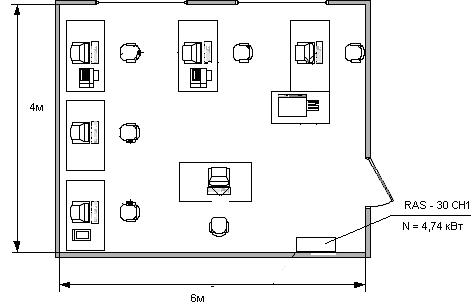
\includegraphics{plan.png}
      \caption{План приміщення}
      \label{fig:plan}
    \end{figure}

    Згідно з п.~2.3. ДСанПіН~3.3.2-007-98 розмір площі для одного робочого
    місця оператора персонального комп’ютера повинен бути не менше $6$~м$^2$,
    а об’єм --- не менше $20$~м$^3$\cite{dsanpin}.
    Довжина кімнати --- $6.0$~м, ширина --- $4.0$~м, висота --- $2.7$~м.
    Отже, площа приміщення складає
      \[
        S = 6 \times 4 = 24~\text{м}^2,
      \]
    а обсяг
      \[
        V = 24 \times 2.7 = 64.8~\text{м}^2.
      \]
    Кожне робоче місце обладнане електронно"=обчислювальними машинами з
    РК"=моніторами Samsung LN32D403E2DXZA.
    У приміщенні постійно працює до чотирьох чоловік.
    Отже, на кожне робоче місце припадає по $6.0$~м$^2$ площі в об’ємі не
    менше, ніж $20.0$~м$^3$, що відповідає санітарним нормам.
  \subsection{Аналіз шкідливих і небезпечних виробничих факторів}
    \subsubsection{Мікроклімат}
    \subsubsection{Шум}
    \subsubsection{Освітлення}
    \subsubsection{Електробезпека}
  \subsection{Пожежна безпека}
  \subsection{Інструкція з техніки безпеки}
    \bibliographystyle{ugost2008ls}
    \bibliography{src}
\end{document}
